\documentclass[11pt]{article}
\usepackage{amsmath,amsthm}
\usepackage{tikz}
\usetikzlibrary{positioning, shapes.misc}
\usepackage{tikz}
\usetikzlibrary{arrows,backgrounds,calc,fit,decorations.pathreplacing,decorations.markings,shapes.geometric}
\tikzset{every fit/.append style=text badly centered}

\begin{document}

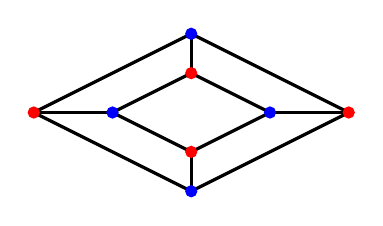
\begin{tikzpicture}[scale=0.5]
        \draw[very thick] (-4,0)--(0,2);
        \draw[very thick] (-4,0)--(-2,0);
        \draw[very thick] (-4,0)--(0,-2);

        \draw[very thick] (4,0)--(0,2);
        \draw[very thick] (4,0)--(2,0);
        \draw[very thick] (4,0)--(0,-2);

        \draw[very thick] (0,1)--(0,2);
        \draw[very thick] (0,1)--(2,0);
        \draw[very thick] (0,1)--(-2,0);

        \draw[very thick] (0,-1)--(0,-2);
        \draw[very thick] (0,-1)--(2,0);
        \draw[very thick] (0,-1)--(-2,0);
        
        \filldraw [blue] (0,2) circle (4pt);
        \filldraw [blue] (0,-2) circle (4pt);
        \filldraw [blue] (2,0) circle (4pt);
        \filldraw [blue] (-2,0) circle (4pt);
        
        \filldraw [red] (-4,0) circle (4pt);
        \filldraw [red] (4,0) circle (4pt);
        \filldraw [red] (0,-1) circle (4pt);
        \filldraw [red] (0,1) circle (4pt);
    \end{tikzpicture}

\end{document}